% !TeX document-id = {1ac77cce-10e1-40ed-b3e7-2d56b8a908ff}
% !TeX root = cloudlab.tex
% !TeX TXS-program:compile = txs:///pdflatex/[--shell-escape]

\documentclass{article}
\usepackage{blindtext}

%%% FONTS %%%
\usepackage[T1]{fontenc}
\usepackage[utf8]{inputenc}
\usepackage[english]{babel}
%\usepackage{tgpagella} % set the document font to TeX Gyre Pagella
%\usepackage{tgbonum} % set the document font to TeX Gyre Bonum
%\usepackage{fontawesome5} % The Creative Commons icons

%%% DRAFT watermark %%%
\usepackage{draftwatermark}
\SetWatermarkText{DRAFT}
\SetWatermarkScale{5.1}
\SetWatermarkLightness{0.8}

\usepackage{xcolor} % \textcolor{red}{text} will be red for notes
\definecolor{lightgray}{gray}{0.6}
\definecolor{medgray}{gray}{0.4}

\usepackage{hyperref}
\hypersetup{
	colorlinks=true,
	urlcolor= blue,
	citecolor=blue,
	linkcolor= blue,
	% bookmarks=true,
	% bookmarksopen=false,
}

% Code to add paragraph numbers and titles
\newif\ifptitle
\newif\ifpnumber
\newcounter{para}
\newcommand\ptitle[1]{\par\refstepcounter{para}
	{\ifpnumber{\noindent\textcolor{lightgray}{\textbf{\thepara}}\indent}\fi}
	{\ifptitle{\textbf{[{#1}]}}\fi}}
\ptitletrue  % comment this line to hide paragraph titles
\pnumbertrue  % comment this line to hide paragraph numbers

% for inserting images in line
\usepackage{graphicx}
\graphicspath{ {images/} }

% Allows to rewrite the same title in the supplement
\newcommand{\mytitle}{A Cloud Based Lab Environment for Network Security Research}
\usepackage{authblk}
\usepackage{comment} % allows block comments

\usepackage{ragged2e} % use flush and justify for text blocks
\usepackage{csquotes} % use \displayquote{} in the doc

%%% GRAPHICS  AND CODE BLOCKS %%%
\usepackage[listings, minted]{tcolorbox}
\usepackage{xcolor}
\definecolor{myblue}{RGB}{0,163,243}
\definecolor{mygrey}{RGB}{128,128,128}
\definecolor{whitesmoke}{RGB}{245,245,245}
\newtcolorbox[auto counter, number within=section]{mybox}[2][]{
	colbacktitle=mygrey,
	colback=whitesmoke,
	title={#2},
	fonttitle=\ttfamily\small,
	fontupper=\sffamily\small,
	halign=flush left,
	rounded corners
}

%\usepackage[verbose]{wrapfig} % wrap text around image

% color table cells
\usepackage[table]{xcolor,colortbl}% http://ctan.org/pkg/xcolor
\definecolor{myblue}{HTML}{4285F4}

% Headers and footers
\usepackage{fancyhdr}
\pagestyle{fancy}
\fancyhf{}
\lhead{A Cloud Native Security Lab}
\lfoot{\tiny{September 7, 2021}}
\rfoot{\tiny{version: 0.1}}


\begin{document}

\title{\mytitle}
\author[1,2]{Franklin E. Diaz\\ \texttt\href{emailto: fdiaz@paloaltonetworks.com}{fdiaz@paloaltonetworks.com}}
\affil[1]{Palo Alto Networks}
\affil[2]{Professional Services - Automation}
\begin{titlepage}
	\date{September 7, 2021}
	\maketitle
	%\thispagestyle{empty} % remove page number from title page? 
	\begin{abstract}
		\raggedright
		The goal of this document is to detail the major components of the ``Cloudlab'' network security lab in
		\href{https://cloud.google.com/}{Google Cloud}. The reasoning behind including certain components and design elements is explained. 
		The relationship between security and the lab are detailed to highlight purpose. Security learning objectives are realized
		at every step of the process in the creation and use of this lab. The result is a widely scoped and highly flexible security
		learning environment for data scientists and engineers with focus on development, test, operations, and continuous pipelines.\\
		\vspace{4cm}
		\centering{\href{https://github.com/devsecfranklin/paper-cloud-lab/blob/main/cloudlab.pdf}{ Click here to download latest version.}}

	\end{abstract}
\end{titlepage}

\begin{comment}
Source files for this paper are available at: \url{https://github.com/devsecfranklin/paper-cloud-lab/}
\end{comment}


\begin{displayquote}
	\emph{Cloud-native technologies empower organizations to build and run scalable applications in modern, dynamic environments such as public,
	private, and hybrid clouds.}
	
	\href{https://www.cncf.io/about/who-we-are/}{Cloud Native Computing Foundation}
\end{displayquote}

\section{\label{sec:Start}A Cloud Native Security Lab}
\vspace{2mm}
\justifying
There is a proliferation of new and constantly evolving Public Cloud providers, tools, tool chains, and whole 
``cloud based'' development and operations ecosystems. There is a need to understand and adapt to the ``GitOps'' paradigm and the
business opportunities this fundamental shift presents. There is no disputing the fact that this shift is well underway\cite{CloudShift}. 

\justifying
The ``Cloudlab'' is a private lab environment for security research, testing, and training. The lab is ``Cloud Native'' in the sense that it
adheres to \href{https://www.cloudbees.com/gitops/what-is-gitops}{GitOps practices}. The GitOps methodology facilitates storage, review, and
maintenance of the lab Infrastructure as Code. The lab is currently comprised of two main Pipelines. The first of these is dedicated to Continuous
Integration. The second pipeline facilitates \href{https://cml.dev/doc}{Continuous Machine Learning}, or CML\cite{books/mit/026233758}.

\justifying
As security practitioners, it is important for us to understand an environment as a precursor to securing it.

\section{\label{sec:Project}Project Goals}
\vspace{2mm}
\justifying
There are several goals related to this project. These goals overlap and interconnect at times. The overarching goal is to understand the composition,
management, and weaknesses of the items listed here.

\begin{raggedright}
	\begin{enumerate}
		\item Provisioning \href{https://docs.paloaltonetworks.com/cn-series.html}{Palo Alto Networks CN-Series firewall} products, integrating
		them with \href{https://www.tigera.io/project-calico/}{Calico} and protecting containerized workloads (Kubernetes ``pods'').
		\item Research containerized deployments, workloads and security.
		\item Demonstrate \href{https://github.com/probot/probot}{``automation bots'' and how they interact with a GitHub repository}. Extending a
		revision control platform (GitHub in this case) is rather common in large organizations.
		\item Integration of \href{https://docs.bridgecrew.io/docs}{Bridgecrew ``Security as Code'' tooling} with GitHub repositories.
		\item Develop and demonstrate ``serverless cloud function'' expertise (GCP Cloud Functions in this case).
		\item Develop and use a cloud native Continuous Integration build pipeline. The output of this pipeline is a Docker image that is stored
		in gcr.io. These images include a fully contained set of tools, documentation and Terraform code for customer deployments.
		\item Demonstrate Policy as Code concepts using \href{https://www.accurics.com/products/terrascan/}{Terratest} and 
		\href{https://kyverno.io/}{Kyverno}.
	\end{enumerate}
\end{raggedright}
\vspace{2mm}

\section{\label{sec:Lab}Lab Configuration Details}
\vspace{2mm}
\justifying
The configuration files and code used to build the lab are stored on GitHub. The lab is running on Google Cloud, one of the ``big three'' public cloud providers.
The lab is intended to serve as a proof of concept as well as provide a teaching and training platform.

\begin{figure}[ht]
  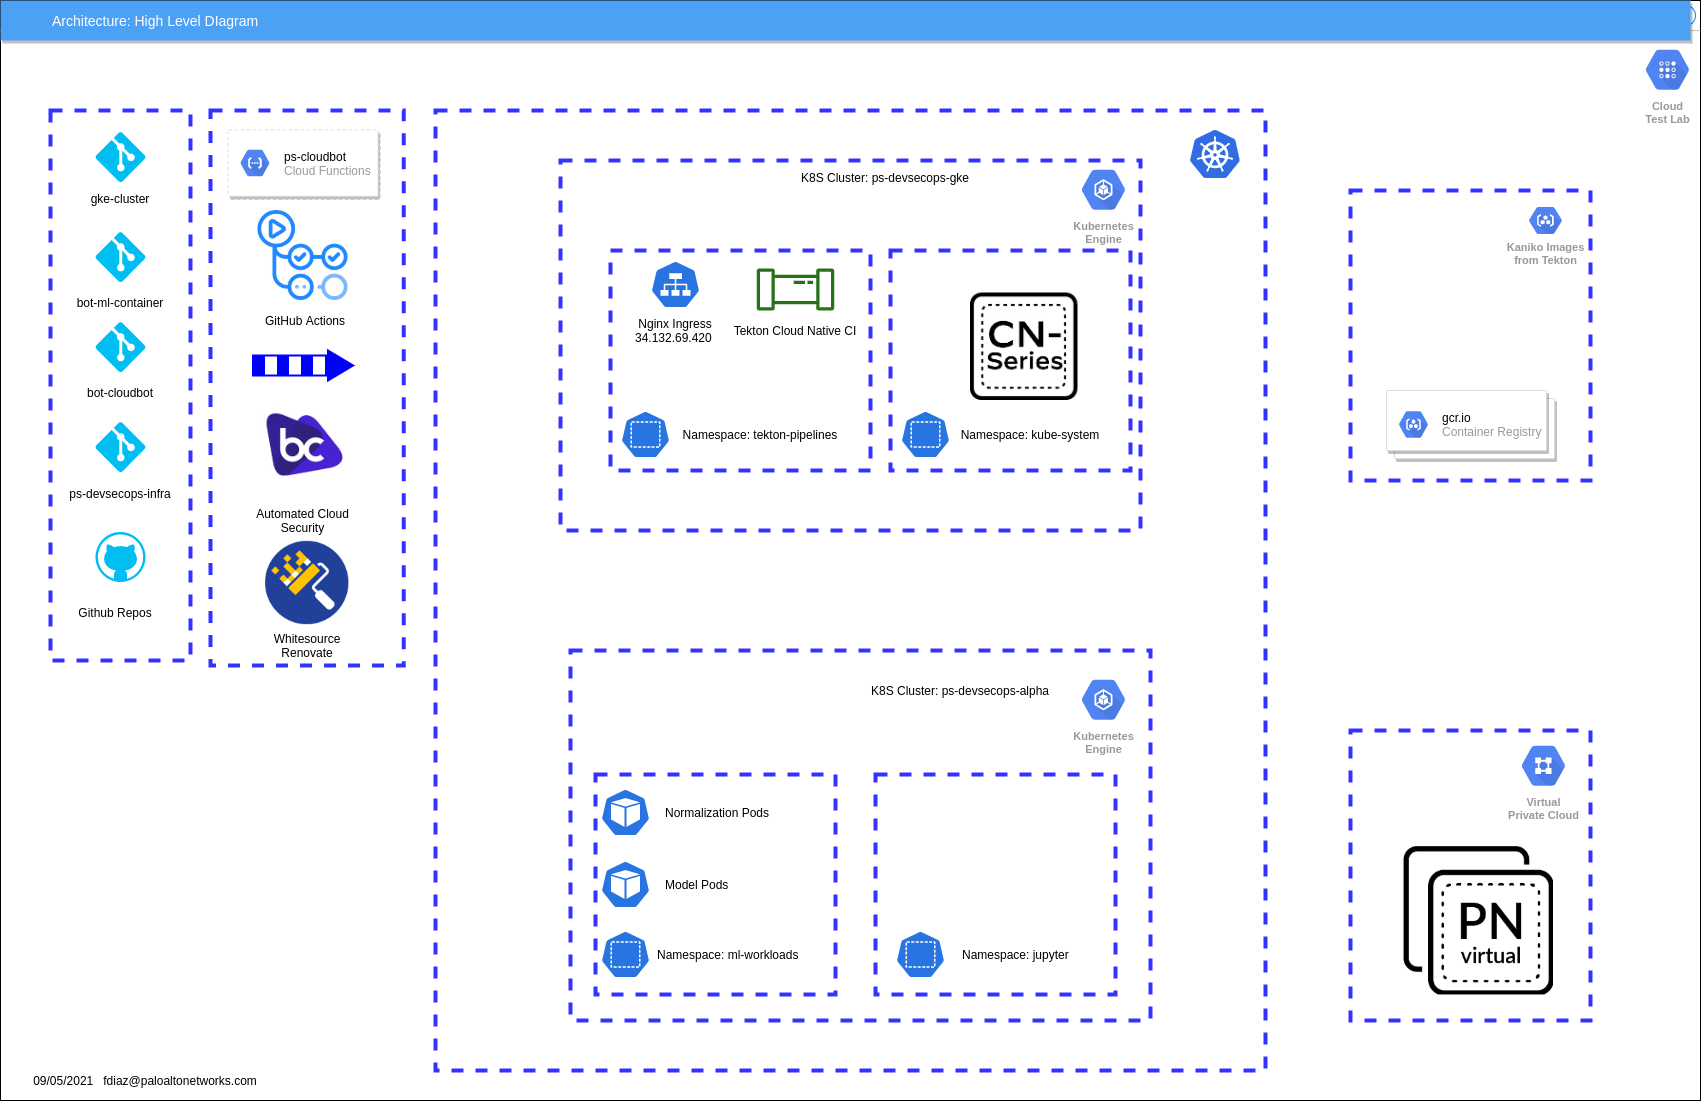
\includegraphics[width=12cm]{cloudlab.png}
  \caption{High Level Lab Design Diagram}
  \label{design}
\end{figure}

\justifying
A detailed description of the five main blocks seen in figure \ref{design} follows.

\newpage
\ptitle{GitHub Repositories}

\justifying
The code base for the lab is broken down into several GitHub repositories, more or less around the functional area. 

\begin{table}[ht]
    \centering
	\begin{tabular}{| p{0.35\linewidth} | p{0.6\linewidth} |} \hline
		\cellcolor{myblue}\textcolor{white}{\textbf{Repo Name}} & \cellcolor{myblue}\textcolor{white}{\textbf{Purpose}} \\\hline
		bot-cloudbot     & A custom Python 3.9 GCP Cloud Function for GitHub pull request task automation.\\\hline
		bot-ml-container & An experimental containerized machine learning model.\\\hline
		gke-cluster      & Infra as Code files for GKE cluster, YAML files for \href{https://tekton.dev/}{Tekton CI pipeline}. CN Series firewall nodes.\\\hline
		ps-containerizer & An `invisible shim'' with a Docker image for each ``public cloud'' VM-Series Terraform module development repo. Allows PRs to be
		ingested into Tekton CI pipeline without any integrations with the source repository.\\\hline
		ps-devsecops-alpha & IaC files for Alpha K8s cluster.\\\hline
		python-project-template & Python project template for writing serverless code in AWS Lambda and GCP cloud functions.\\\hline
	\end{tabular}
	\caption{Project Codebase - GitHub Repositories}
    \label{mytable:1}
\end{table}
\vspace{2mm}
\ptitle{GitHub Actions}
\vspace{2mm}
\justifying
GitHub repositories that have been "on-boarded" to the project have certain ``actions'' included.

\begin{raggedright}
	\begin{enumerate}
        \item \href{https://docs.bridgecrew.io/docs}{Bridgecrew} is used to scan all commits to all open pull requests.
        \item Whitesource Renovate is used to track keep project dependencies up to date and secure.
        \item Another GitHub action defines the parameters of the GCP project and helps the ``ps-cloudbot'' with pull request  maintenance tasks.
	\end{enumerate}
\end{raggedright}
\vspace{2mm}

\justifying
Note that there is also a \href{https://docs.github.com/en/developers/webhooks-and-events/webhooks/about-webhooks}{webhook} to make the CI pipeline
aware of each commit and kick off a test and build cycle.
\vspace{2mm}
\justifying
\ptitle{Kubernetes Clusters}
\vspace{2mm}
\justifying
Two clusters are deployed with the Google Kubernetes Engine (GKE). The ``gke'' cluster hosts the Tekton CI pipeline.
The ``alpha'' cluster is used for machine learning experimentation.

\justifying
Pipeline runs can be viewed and managed through a graphical interface that is well suited for development teams. There is
also the ability to manage pipeline runs and their requisite tasks using standard command line tooling.

\begin{mybox}{\thetcbcounter: Example pipeline command}
	\lstinputlisting{code/tkn-run.txt}
\end{mybox}
\vspace{2mm}
\ptitle{GCR Private Container Repository}
\vspace{2mm}
\justifying
To date there are about 15 GitHub repositories that are integrated with the CI pipeline outlined in this paper. Each commit
to a pull request causes the CI pipeline to generate a Docker image. These Docker images 
are \href{https://cloud.google.com/container-registry/}{stored in a private GCR location}.
\vspace{2mm}
\ptitle{Panorama Management}
\vspace{2mm}
\justifying
Panorama is a key component in deployment and maintenance of Kubernetes clusters and CN Series firewalls. Currently we have
two virtual Panorama devices deployed in a high availability (HA) configuration.

\justifying
Palo Alto networks has historically maintained serverless functions, for example in AWS Lambda, for firewall ``auto-scaling'' tasks. This has since been
replaced by a set of official Panorama ``plug-ins'' that can be downloaded to PanOS devices. Lambda and Cloud functions
are still frequently used to augment the capabilities of this new family of plug-ins.
\vspace{2mm}
\section{\label{sec:LO}Learning Objectives}
\vspace{2mm}
Building and operating this lab is meant to foster learning. It may be beneficial for engineers to focus on some or all of the
following list of topics.

\begin{raggedright}
	\begin{enumerate}
		\item Deployment and operation of CN Series firewalls.
		\item Kubernetes role based access control (RBAC) and security.
		\item Developing serverless functions in Python.
		\item ML/AI pipeline, containerized workloads, and their security.
		\item Containers and container security.
		\item Automation.
		\item Testing perspectives including Policy as Code, Security as Code, etc.
		\item CI/CD Pipelines and security.
	\end{enumerate}
\end{raggedright}
\vspace{2mm}

Training materials derived from lab construction and operation are easily within reach of PS engineers. 

\section{\label{sec:CI}Continuous Integration}

Keeping internal and external build pipelines secure, as well as scanning work products that traverse these pipelines is highly desirable. To that end, a
fully operational Cloud Native Continuous Integration pipeline has been implemented in the lab.

The pipeline can ingest a code base from a public repo, or a private repo with proper credentials. The ``containerizer'' repo demonstrates the ability
to collect files from a repository, bundle it with requisite command line tools, test cases, and other necessities, and ship the image to the gcr.io container
registry at the conclusion of a successful pipeline run. a pipeline run refers to a set of test cases managed and executed by Tekton.

\begin{figure}[ht]
	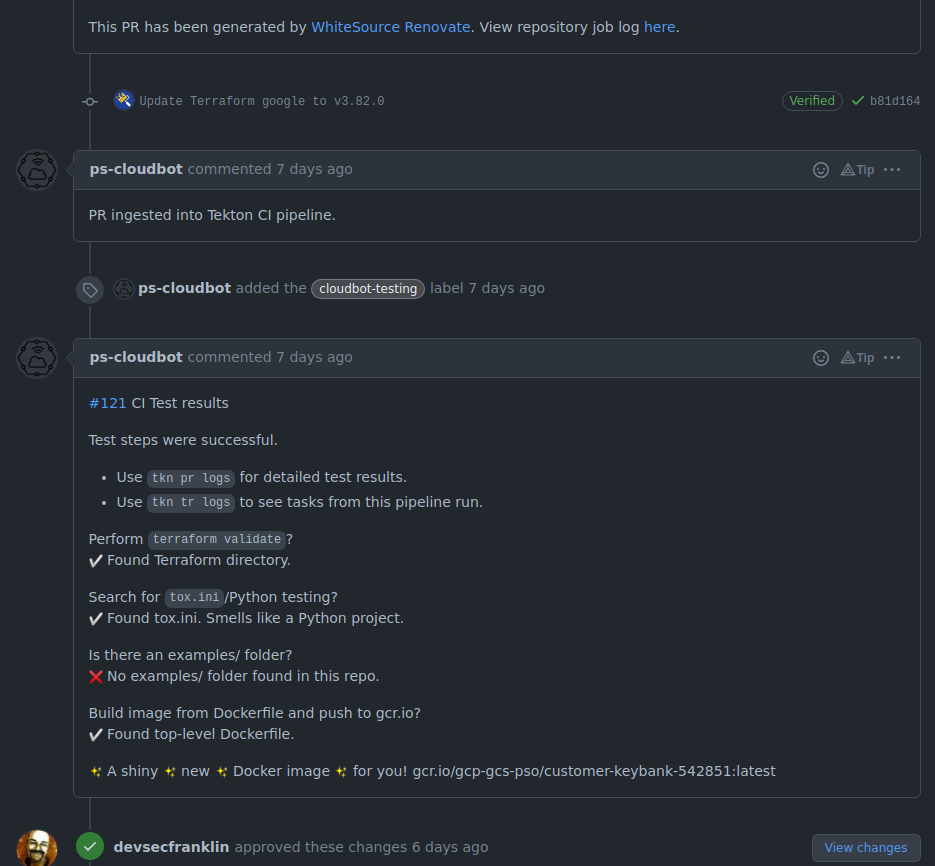
\includegraphics[width=12cm]{pr1.png}
	\caption{Tekton automated pipeline run results in a GitHub comment}
	\label{pr}
\end{figure}

Consider figure \ref{pr}. The ``Renovate'' bot detects an out of date or insecure dependency. A pull request is opened by the Renovate bot. 
Next, ``ps-cloudbot'' GCP cloud function is notified of the new pull request via webhook. The second bot places a label on the pull request to indicate
it is performing administrative actions on the pull request. The cloud function might perform other actions such as assigning the pull request to a certain user,
adding certain users as reviewers, providing documentation, and so on. In this example, the cloud function adds a comment to the pull request to inform
project members that it has been accepted by the CI pipeline. A set of test cases based on certain technology or functional area is executed and the
results are returned to the pull request in a second comment. There is also a link to the container image in the container registry. Although the pull
request is merged manually in this instance, the workflow could be modified to approve and merge the pull request with no human interaction whatsoever.

\begin{figure}[ht]
	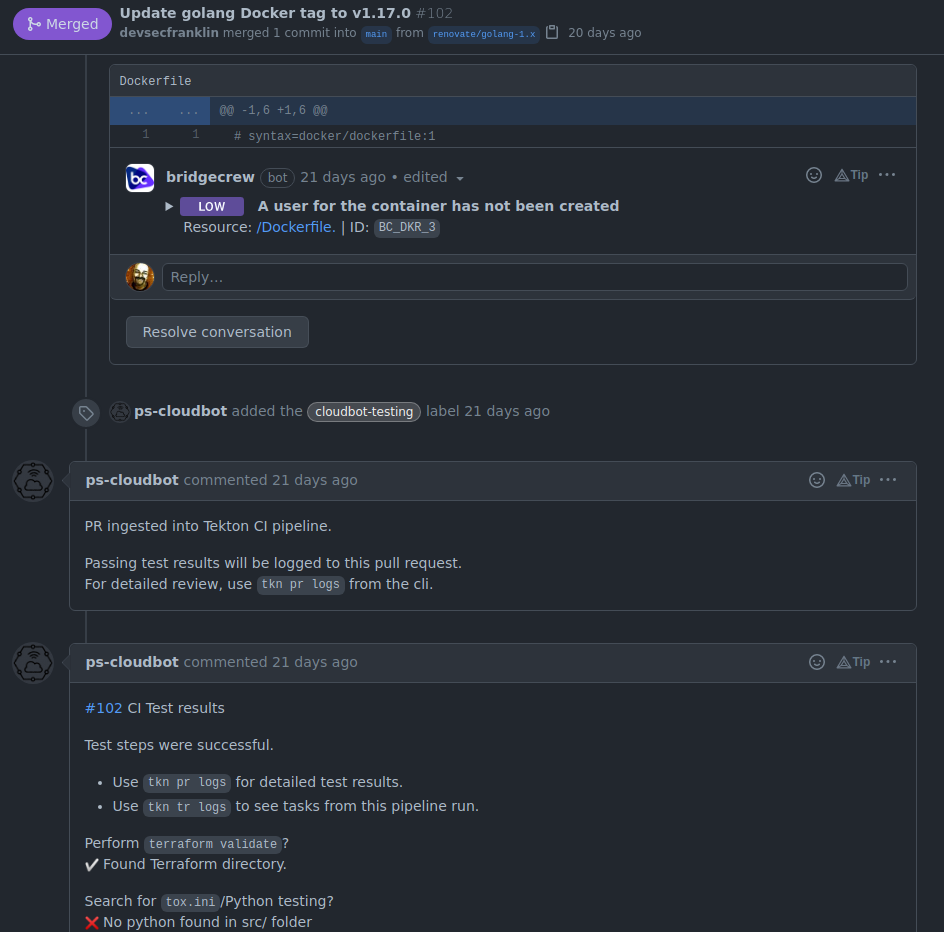
\includegraphics[width=12cm]{pr2.png}
	\caption{Bridgecrew integration with pull request automation}
	\label{pr2}
\end{figure}

In addition to the ability to scan for dependencies which are out of date or have vulnerabilities of note, we can perform automated security scanning
of the code base as seen in figure \ref{pr2}. As before, the Renovate bot has detected the use of an out of date Docker base image for Golang. Because
the Dockerfile is updated as part of this pull request, \href{https://docs.bridgecrew.io/docs}{Bridgecrew} scans the file and triggers on misconfigurations that may lead to security issues.
The results of the scans and the issues are noted in the pull request comments. Automated remediation and merging of these issues may be possible in
some cases.



\section{\label{sec:Summary}Summary}
\vspace{2mm}
Future goals for the lab project might include, but are not limited to the following list.
\vspace{2mm}
\begin{raggedright}
	\begin{enumerate}
		\item Orchestration of Multi-Cloud infrastructure builds and deployments, \href{https://crossplane.io/docs/v1.3/}{using Crossplane for example}.
		\item Understanding infrastructure as code in languages besides HCL (aka Terraform). One example of this is \href{https://www.pulumi.com/}{Pulumi}.
		\item ``Red teaming'' our own lab, conducting dynamic application security testing (DAST) exercises.
	\end{enumerate}
\end{raggedright}
\vspace{2mm}

\nocite{*}
\bibliographystyle{plain}
\bibliography{mybib.bib}

\end{document}
